\documentclass[twoside]{homework}

% for bar over variable
\newcommand*\conj[1]{\overline{#1}}
\newcommand*\mean[1]{\overline{#1}}

% for graph
\usepackage{pgfplots}
\usepackage{enumerate}
% for double stroke 1
\usepackage{bbm}

% for < and >
\usepackage[T1]{fontenc}

% for equation wrap text
\usepackage{amsmath}
\usepackage{bm}

\studname{Kangwei Ling}
\studmail{kl3076@columbia.edu}
\coursename{CSOR 4231, Section 3: Analysis of Algorithms I}
\hwNo{2}
\begin{document}
\maketitle
\subsubsection*{Collaborators}
Zefeng Liu (zl2715), Kunyan Han (kh2931), Luoyao Hao (lh2913).
\section{DPV 2.12}
Let $L(n)$ be the total numbers of lines printed, according to the description, we have
\[ L(n) = 2L(n/2) + 1, L(1) = 0\]
Using the master theorem, $L(n) = \Theta(n)$

\section{DPV 2.8 and 2.9}
\subsection*{2.8}
\begin{enumerate}
	\item [(a)] There are 4 coefficients, choose $\omega = e^{2\pi i/4} = i$. Thus:
		\[FFT((1, 0, 0, 0), \omega) = \begin{bmatrix}
			1 & 1 & 1 & 1 \\
			1 & \omega & \omega^2 & \omega^3 \\
			1 & \omega^2 &\omega^4 & \omega^6 \\
			1 & \omega^3 &\omega^6 & \omega^9
		\end{bmatrix} \begin{bmatrix}
			1 \\ 0\\ 0\\ 0
		\end{bmatrix}
		= \begin{bmatrix}
			1 \\ 1 \\ 1 \\ 1
		\end{bmatrix}
		\]
		To find out which sequence is $(1,0,0,0)$ the FFT, we calculate the inverse FFT:
		\[\frac{1}{4}FFT((1,0,0,0), w^{-1}) = \frac{1}{4}\begin{bmatrix}
			1 & 1 & 1 & 1 \\
			1 & \omega^{-1} & \omega^{-2} & \omega^{-3} \\
			1 & \omega^{-2} &\omega^{-4} & \omega^{-6} \\
			1 & \omega^{-3} &\omega^{-6} & \omega^{-9}
		\end{bmatrix} \begin{bmatrix}
			1 \\ 0\\ 0\\ 0
		\end{bmatrix}
		= \begin{bmatrix}
			1/4 \\ 1/4 \\ 1/4 \\ 1/4
		\end{bmatrix}\]
	\item [(b)] choose the same $\omega = i$.
	\[FFT((1, 0, 1, -1), \omega) = \begin{bmatrix}
		1 & 1 & 1 & 1 \\
		1 & i & -1 & -i \\
		1 & -1 & 1 & -1 \\
		1 & -i & -1 & i
	\end{bmatrix} \begin{bmatrix}
		1 \\ 0\\ 1\\ -1
	\end{bmatrix}
	= \begin{bmatrix}
		1 \\ i \\ 3 \\ -i
	\end{bmatrix}
	\]

	To find out which sequence is $(1,0,1,-1)$ the FFT, we calculate the inverse FFT:
	\[\frac{1}{4}FFT((1,0,1,-1), w^{-1}) = \frac{1}{4}\begin{bmatrix}
		1 & 1 & 1 & 1 \\
		1 & -i & -1 & i \\
		1 & -1 & 1 & -1 \\
		1 & i & -1 & -i
	\end{bmatrix} \begin{bmatrix}
		1 \\ 0\\ 1\\ -1
	\end{bmatrix}
	= 1/4\begin{bmatrix}
		1 \\ -i \\ 3 \\ i
	\end{bmatrix}\]
\end{enumerate}
\subsection*{2.9}
\begin{enumerate}
	\item [(a)] $x+1 = 1 + x + 0x^2 + 0x^3$, we represent this polynomial with $(1, 1, 0, 0)$.

	$x^2 + 1 = 1 + 0x + 1x^2 + 0x^3$, represented as $(1, 0, 1, 0)$.

	Since $n = 4$, $\omega = e^{2\pi i/4} = i$. The FFT of these two sequence is:
	\[FFT((1, 1, 0, 0), \omega) = \begin{bmatrix}
		1 & 1 & 1 & 1 \\
		1 & i & -1 & -i \\
		1 & -1 & 1 & -1 \\
		1 & -i & -1 & i
	\end{bmatrix} \begin{bmatrix}
		1 \\ 1\\ 0\\ 0
	\end{bmatrix}
	= \begin{bmatrix}
		2 \\ 1 + i \\ 0 \\ 1 - i
	\end{bmatrix}
	\]

	\[FFT((1, 0, 1, 0), \omega) = \begin{bmatrix}
		1 & 1 & 1 & 1 \\
		1 & i & -1 & -i \\
		1 & -1 & 1 & -1 \\
		1 & -i & -1 & i
	\end{bmatrix} \begin{bmatrix}
		1 \\ 0\\ 1\\ 0
	\end{bmatrix}
	= \begin{bmatrix}
		2 \\ 0 \\ 2 \\ 0
	\end{bmatrix}
	\]
	multiply the two results, we have the values $(4, 0, 0, 0)$. Then the inverse FFT:
	\[\frac{1}{4}FFT((4,0,0,0), w^{-1}) = \frac{1}{4}\begin{bmatrix}
		1 & 1 & 1 & 1 \\
		1 & -i & -1 & i \\
		1 & -1 & 1 & -1 \\
		1 & i & -1 & -i
	\end{bmatrix} \begin{bmatrix}
		4 \\ 0 \\ 0 \\ 0
	\end{bmatrix}
	= \begin{bmatrix}
		1 \\ 1 \\ 1 \\ 1
	\end{bmatrix}\]
	Therefore the final result is $1 + x + x^2 + x^3$.

	\item [(a)] $1 + x + 2x^2 = 1 + x + 2x^2 + 0x^3$, we represent this polynomial with $(1, 1, 2, 0)$.

	$2 + 3x = 2 + 3x + 0x^2 + 0x^3$, represented as $(2, 3, 0, 0)$.

	Since $n = 4$, $\omega = e^{2\pi i/4} = i$. The FFT of these two sequence is:
	\[FFT((1, 1, 2, 0), \omega) = \begin{bmatrix}
		1 & 1 & 1 & 1 \\
		1 & i & -1 & -i \\
		1 & -1 & 1 & -1 \\
		1 & -i & -1 & i
	\end{bmatrix} \begin{bmatrix}
		1 \\ 1 \\ 2 \\ 0
	\end{bmatrix}
	= \begin{bmatrix}
		4 \\ -1 + i \\ 2 \\ -1 -i
	\end{bmatrix}
	\]

	\[FFT((2, 3, 0, 0), \omega) = \begin{bmatrix}
		1 & 1 & 1 & 1 \\
		1 & i & -1 & -i \\
		1 & -1 & 1 & -1 \\
		1 & -i & -1 & i
	\end{bmatrix} \begin{bmatrix}
		2 \\ 3\\ 0\\0
	\end{bmatrix}
	= \begin{bmatrix}
		5 \\ 2 + 3i \\ -1 \\ 2 - 3i
	\end{bmatrix}
	\]
	multiply the two results, we have the values $(20, -5-i, -2, -5+i)$. Then the inverse FFT:
	\[\frac{1}{4}FFT((20,-5-i,-2,-5+i), w^{-1}) = \frac{1}{4}\begin{bmatrix}
		1 & 1 & 1 & 1 \\
		1 & -i & -1 & i \\
		1 & -1 & 1 & -1 \\
		1 & i & -1 & -i
	\end{bmatrix} \begin{bmatrix}
		20 \\ -5-i \\ -2 \\ -5+i
	\end{bmatrix}
	= \begin{bmatrix}
		2 \\ 5 \\ 7 \\ 6
	\end{bmatrix}\]
	Therefore the final result is $2 + 5x + 7x^2 + 6x^3$.
\end{enumerate}

\section{DPV 2.27}
\begin{enumerate}
	\item [(a)] Let $A = \begin{bmatrix}
		a_0 & a_1 \\ a_2 & a_3
	\end{bmatrix}$, then $A^2 = \begin{bmatrix}
		a_0^2 + a_1a_2 & a_0a_1 + a_1a_3 \\ a_0a_2 + a_2a_3 & a_1a_2 + a_3^2
	\end{bmatrix}$

	By inspection, $A^2 = \begin{bmatrix}
		a_0^2 + M && a_1N \\ a_2N && M + a_3^2
	\end{bmatrix}$, where $M = a_1a_2, N = a_0 + a_3$, now only 5 multiplications are sufficient to compute $A^2$.

	\item [(b)] Using the same notation for a $n\times n$ matrix $M$, we write $M = \begin{bmatrix}
		A & B \\ C & D
	\end{bmatrix}$
	where $A, B, C, D$ are all $n/2 \times n/2$ matrices (assume $n$ is even).
	In this case,
	\[M^2 = \begin{bmatrix}
		A^2 + BC & AB + BD \\ CA + CD & CB + D^2
	\end{bmatrix}\]
	By dividing the problem, we cannot get 5 subproblems as we get 5 multiplications for $2\times 2$ matrix, because for scalars it holds that $a_0a_1 + a_1a_3 = a_2(a_0 + a_3)$, while for matrices, $AB + BD = B(A + D)$ does not always hold since $AB$ is not equivalent to $BA$.

	\item [(c)]
		\begin{enumerate}
			\item [i.] Note that, $(A+B)^2 = A^2 + B^2 + AB + BA$, so $AB +BA = (A+B)^2 - A^2 - B^2$, addition and subtraction of these matrices can be done in $O(n^2)$. If $n\times n$ matrices can be squared in time $S(n) = O(n^c)$, then we can compute $AB+BA$ in time $3S(n) + O(n^2)$.
			\item [ii.] \[ AB + BA = \begin{bmatrix}
				0 & XY \\ 0 & 0
			\end{bmatrix} + \begin{bmatrix}
				0 & 0 \\ 0 & 0
			\end{bmatrix} = \begin{bmatrix}
				0 & XY \\ 0 & 0
			\end{bmatrix}_{2n \times 2n}\]

			\item [iii.] Given conclusions and results in i. and ii., for two $n\times n$ matrices $X, Y$, we can embed them in $2n \times 2n$ matrices $A, B$ (as described in ii.), the result of $XY$ is in matrix $AB + BA$, which can be computed in time $3S(2n) + O(n^2)$. Therefore the product $XY$ can be computed in time $3S(2n) + O(n^2) = 3\times 2^c O(n^c) + O(n^2) = O(n^c) + O(n^2) = O(n^c)$ (since we are consider possible $c < \log_2 7$, also $c > 2$ for sure).
		\end{enumerate}
\end{enumerate}

\section{DPV 3.14}
A linear time algorithm goes as follow (assume the graph is represented by adjacency list):

\begin{enumerate}
	\item First, scan all edges. For each edge $e = (u, v)$, we increase the indegree(initialized to 0) of vertex $v$ by 1.
	\item Second, go through the indegrees of each vertex, add a vertex to $sources$ (a list that contains all source vertices) if it has indegree of 0.
	\item We loop until the $sources$ list is empty, in each iteration, we pick one vertex $v$ from the $sources$ list and remove it from the list. This vertex is emitted. Then for each edges goes out from $v$, $e = (v, w)$, we decrease the indegree of $w$, if the indegree of $w$ reaches 0, we also add it to the $sources$ list.
	\item When the loop ended, every vertex is emitted in a linearized order. Otherwise the graph is not topological sortable.
\end{enumerate}
Note that 1. 2. 3. all run in linear time, for 3., each vertex will be in the $sources$ list once and each iteration will remove one vertex from the list.

Therefore we have a linear time algorithm for linearization (topological sorting).

\section{DPV 3.2}
\begin{enumerate}
	\item [(a)] See below.

		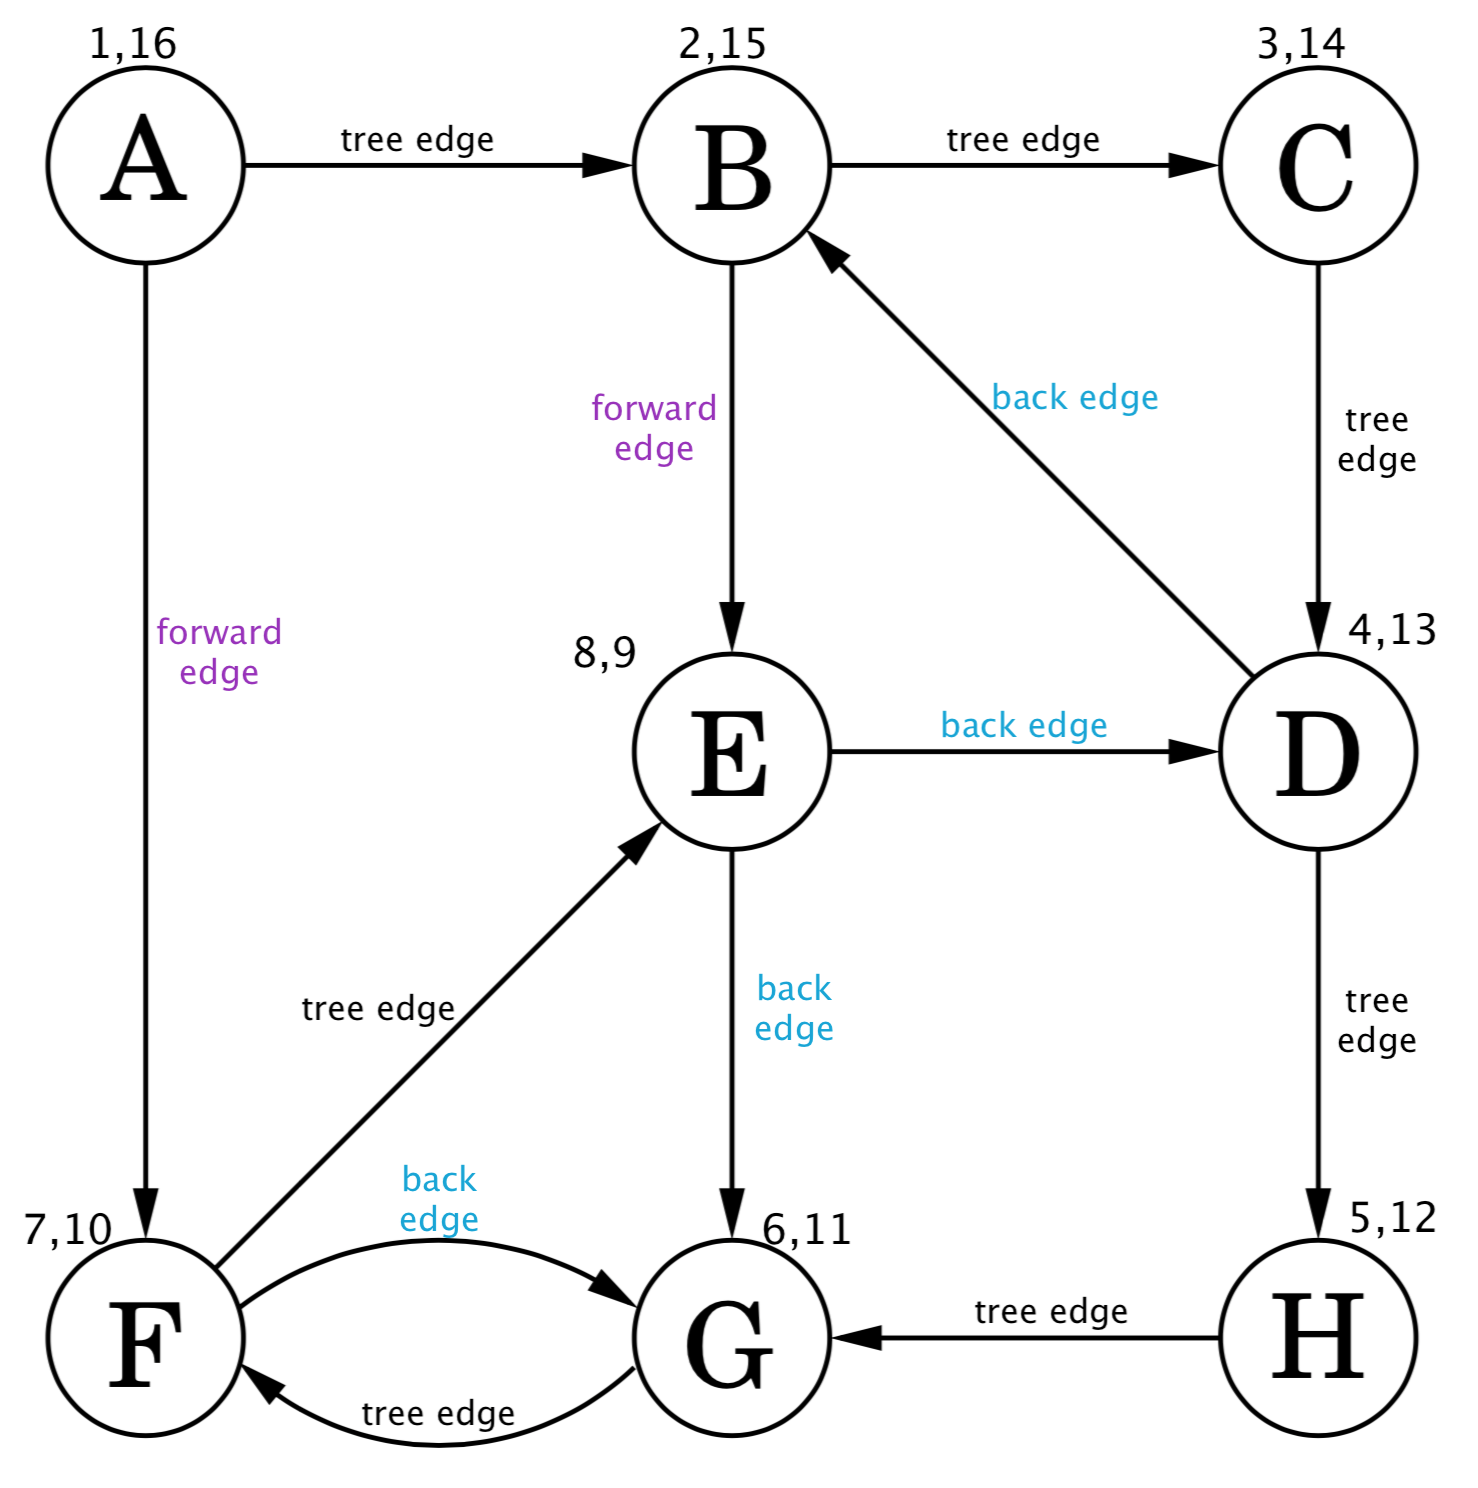
\includegraphics[width=.5\textwidth]{5a.png}
	\item [(b)] See below.

		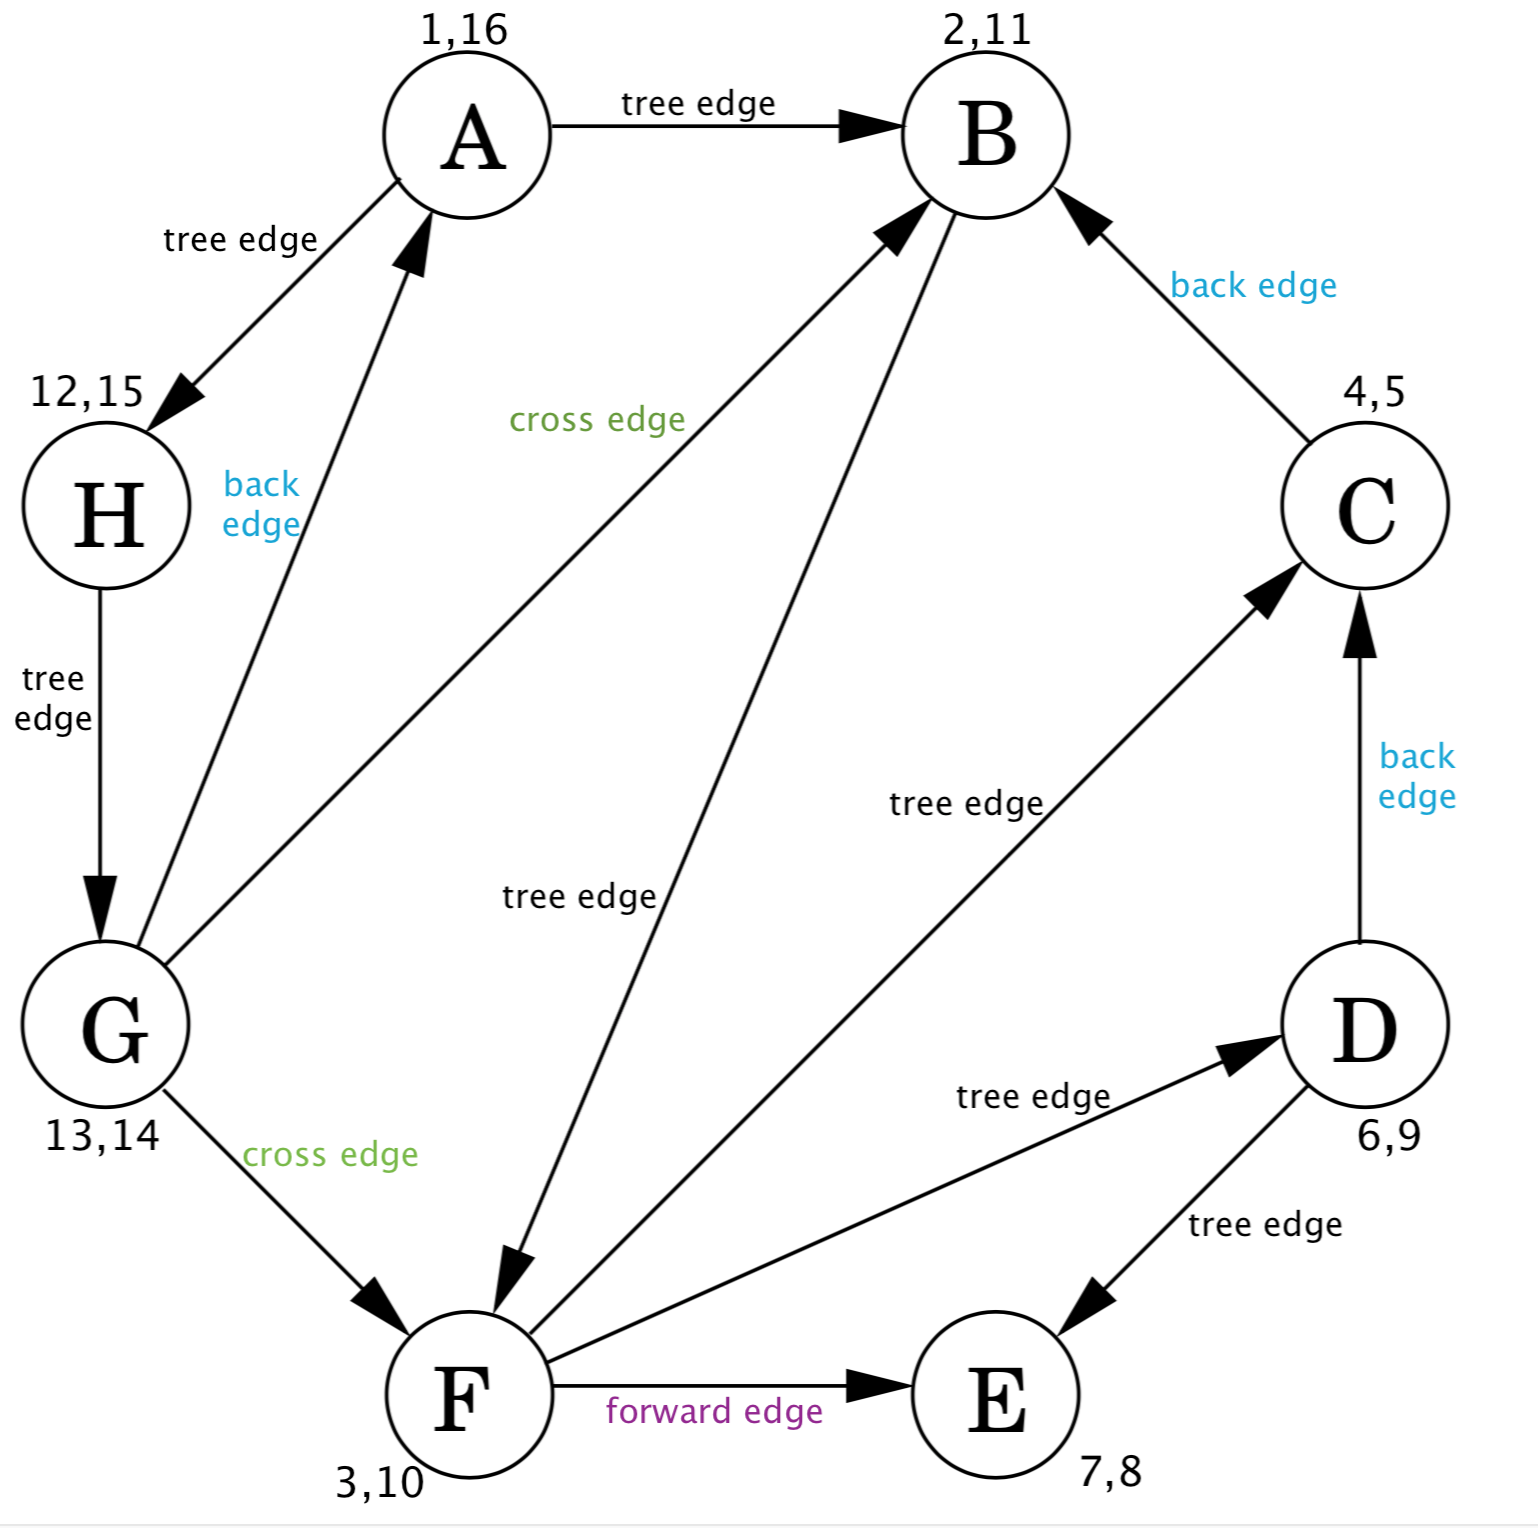
\includegraphics[width=.5\textwidth]{5b.png}
\end{enumerate}

\section{}
\begin{enumerate}
	\item [(a)]
	\begin{proof}
		Let $f$ be any $monotone function$ in the grid $G(d, n)$.

		Let $x_0 = (0, 0, ...,0)$, if $f(x_0) = (0,0,...,0) = x_0$, then $x_0$ is a fix point for $f$, we are done.

		If $f(x_0) = x_1 \neq x_0$, then it must be true that $x_1 > x_0$, because according to the definition, in $G(d, n)$, $x_0$ is the minimum (each component of $x_0$ is 0). Thus $f(x_1) \geq f(x_0)$, i.e., $f(x_1) = x_2 \geq x_1$. Then we can know that $x_3 = f(x_2) \geq f(x_1) = x_2$. In this manner, it is trivial to see that
		\begin{align*}
			x_2 = f(x_1) &\geq f(x_0) = x_1 \\
			x_3 = f(x_2) &\geq f(x_1) = x_2 \\
			x_4 = f(x_3) &\geq f(x_2) = x_3 \\
				&\cdots \\
			x_i = f(x_{i-1})&\geq f(x_{i-2}) = x_{i-1}
		\end{align*}
		There must be some point $x_k$ in this sequence, s.t. $f(x_k) = x_k$. I'll prove by contradiction. If no such $x_k$ exists, then we can keep calculate $x_i$ based on $x_{i-1}$:
		\begin{align*}
			x_2 = f(x_1) &> f(x_0) = x_1 \\
			x_3 = f(x_2) &> f(x_1) = x_2 \\
			x_4 = f(x_3) &> f(x_2) = x_3 \\
				&\cdots \\
			x_i = f(x_{i-1})&> f(x_{i-2}) = x_{i-1} \\
			&\cdots
		\end{align*}
		where $x_i> x_{i-1}$ is defined as at least 1 component of $x_i$ is larger than $x_{i-1}$'s components and other components stay equal.
		since $x_i > x_{i-1}$, there is at least one component of $x_i$ that is larger than the corresponding component of $x_{i-1}$. We cannot increase components of $x_i$ infinitely, because the maximum we can have here is $(n-1, n-1, ..., n-1)$. Therefore, at some point $x_k$, we must have that $x_{k+1} = f(x_k) = f_(x_{k-1}) = x_k$. That $x_k$ is a fix point of $f$.
		\end{proof}
		\item [(b)] \begin{proof}
			In the proof of (a), we keep calculating $x_i$ with the formula $x_{i+1} = f(x_{i})$. In each step, we calculate $x_{i+1} = f(x_i)$, if $x_{i+1} = f(x_i) = x_i$, then we find our fixpoint. Otherwise we go next step with $x_{i+2}$ base on $x_{i+1}$. Note that if $x_{i+1} = f(x_i) \neq x_i$, then at least one component of $x_{i+1}$ is at least 1 larger than that component of $x_i$ ($x_{i+1} > x_i$). If we don't see any fixpoint and we keep going on, then we run into $x_k = (n-1, n-1,...,n-1)$, at this point, it must hold that $x_{k+1} = f(x_k) = x_k$, because there exists no such d-tuple $x'$ in $G(d, n)$ s.t. $x' > x_k = (n-1, n-1, ..., n-1)$.

			The maximum number of steps we can do until we get $(n-1, n-1, ..., n-1)$ is $O(nd)$. In each step, we only need to evaluate $f$ on $x_i$ and compare $f(x_i)$ with $x_i$, which can be done in $O(1)$. Therefore a fixpoint can be found in time $O(nd)$.
		\end{proof}

	\item [(c)]
		\begin{enumerate}
			\item [i)] When $d=1$, $x_0 = 0$, $x_{max} = n-1$, also, $f(x_0) = f(0) \geq 0, f(x_{max}) = f(n-1) \leq n-1$. We can use binary search to find a fix point in such case.

			Note that,
				for any $0 \leq l \leq h \leq n-1$, if $f(l) \geq l, f(h) \leq h$, then there exists a fixpoint in $[l, h]$.
			This can be proved by induction.
			\begin{itemize}
				\item This is obvious if $l = h$.
				\item It $h = l + 1$, either $f(l) = l$ or $f(h) = h$ must holds because otherwise $f(h) \geq f(l) \geq l + 1 > l$, it will make $f(h) \geq h$, but $f(h) < h$.
				\item If $h > l$, this also holds when $f(l) = l$ or $f(h) = h$. Otherwise the case is $f(l) \geq l+1 > l$ and $f(h) < h$, then $f(l+1) \geq f(l) \geq l+1$, we reduce it to $[l+1, h]$, which holds by induction hypothesis.
			\end{itemize}

			\textbf{Binary Search:}\\
			In each step, we find the midpoint $m = l + \frac{(h - l + 1)}{2}$, where initialy $l = 0, h = n - 1$. At any step, $f(l) \geq l, f(h) \leq h$ (this holds for $0,n-1$).

			If $f(m) = m$, then we are done.

			If $f(m) > m$, then there must exist a fixpoint $k$ in $[m+1, h]$ because $f(m + 1) \geq f(m) \geq m + 1 > m$. We set $l = m + 1$

			If $f(m) < m$, a fixpoint is in $[l, m-1]$, because $f(m-1) \leq f(m) \leq m-1 < m$. We set $h = m-1$.


			The \textbf{Binary Search} method can find the fixpoint in $\log n$ time.

			\item [ii)] Let $p^{(k)}$ be the fix point (ignore the last coordinate)we can get by solving for $G(d-1, n)$ with $x_d = k$ fixed.
			\[ p^{(k)} = (p^{(k)}_1, ..., p^{(k)}_{d-1}, k)\]
			By definition:
			\[f(p^{(k)}) = (p^{(k)}_1, ..., p^{(k)}_{d-1}, k')\]
			Also, let $f_i(x)$ be the $i$ th component of $f(x)$, i.e.
			\[ f_d(p^{(k)}) = k', p_d^{(k)} = k\]

			\textbf{Assumption:} If we view $f_d(p^{(k)})$ as a function: $G(1, n) \rightarrow G(1, n)$, I'll assume it is monotone here.


		\newcommand{\pl}{\ensuremath{p^{(l)}}}
		\newcommand{\ph}{\ensuremath{p^{(h)}}}
		\newcommand{\fpl}{\ensuremath{f_d(p^{(l)})}}
		\newcommand{\fph}{\ensuremath{f_d(p^{(h)})}}
		\newcommand{\fpm}{\ensuremath{f_d(p^{(m)})}}
			Now I'll prove something similar to i):
			\begin{align*}
			&\text{for any } 0 \leq l \leq h \leq n-1, \\
			&\text{if } \fpl \geq l, \fph \leq h, \\
			&\text{then there exists a fixpoint for } f \text{ with the last coordinate in } [l, h]
		\end{align*}
		\begin{itemize}
			\item if $l = h$, we have $\fpl = l$, which means $\fpl = \pl$, then this is a fixpoint we are looking for.
			\item if $h = l + 1$, either $\fpl = l$ or $\fph = h$ must holds because otherwise $\fph \geq\fpl \geq l+1 > l$, it will make $\fph \geq h$, but $\fph < h$.
			\item If $h > l$, this also holds when $\fpl = l$ or $\fph = h$. Otherwise the case is $\fpl \geq l+1 > l$ and $fph < h$, then $f_d(p^{(l+1)}) \geq \fpl \geq l+1$, we reduce it to $[l+1, h]$, which holds by induction hypothesis.
		\end{itemize}

		Then we can use binary search similar to i) to find the right fix point where $f_d(p^{(x_d)}) = x_d$.
		\end{enumerate}
\end{enumerate}



%\underline{Citation:} Please cite any sources you used for this problem.
\end{document}